\chapter{Implementation}\label{ch:implementation}

\section{Presentation and reverse proxy}\label{sec:reverse-proxy}
The second core submodule created for the purpose of collecting the data from the users is the frontend application served over the internet. This can be split further into two different functional modules~--- client and server-side.

\subsection{Client side module}\label{subsec:client-side-module}
The client-side module is an end-user presentation layer that is built with the HTML5\footnote{\url{https://html5.org/}}~and~CSS3\footnote{\url{https://www.w3.org/Style/CSS/Overview.en.html}}~--- technologies that are the core and standard for modern web applications nowadays.
HTML is a widely used markup language used to create hypertext documents and CSS is used as a style-sheet for adding the design for web documents.
The content of the website is taken as a free, prebuilt template taken from the Colorlib\footnote{\url{https://colorlib.com/}} collection.
Offered web templates are licensed under the CC BY 3.0 License \footnote{Creative Commons Attribution 3.0 License --- \url{https://creativecommons.org/licenses/by/3.0/}}.
The mechanism that collects users' mouse actions is designed as a "plugin" script, meaning that the template can be changed easily, so different styled environments that serve various purposes can be used to collect the data.

To use the system and participate in the research, interested user is required to first accept the consents of usage of the website as well as accept the usage of the cookies.
After that, the register option is allowed and required.
Next, the user is redirected to the login page.
To persists consistency of the registration and login, the custom static web pages were created to be easily transferable between the templates.
On each document, the FAQ panel with more information regarding the project is exposed as a drop-down list.
To authenticate, users are required to provide the credentials to log in to the system.
These credentials are then sent through https --- which means that they are secured and encrypted --- to the reverse proxy server which then performs some action to authenticate a user (more on that on the subsection \ref{subsec:server-side-module}), sets the cookie with granted JWT\footnote{\url{https://jwt.io/}} token and redirects the user to the homepage.
The whole sequence is described and shown in \mbox{Fig.~\ref{fig:jwt-sequence}}.

After successful login, the token allows for site usage and ensures the identity of the user.
From now on, the actions performed by user are recorded into the batches and sent to the API every two seconds.
The event listeners are awaiting for four different action types: mouse move, mouse-down, mouse-up, mouse wheel action.
Collected actions are packed into JSON object and sent to the server side API (described in \ref{subsec:server-side-module}) --- the fields included are shown in the Listing~\ref{listing:mouse-events-json-schema}.

\lstinputlisting[language=json, caption=JSON schema for mouse event batches, label=listing:mouse-events-json-schema]{resources/mouse-event-json-schema.json}



% Propably should be included elsewhere, maybe appendix?
\begin{figure}[!hbt]
    
    \centering
    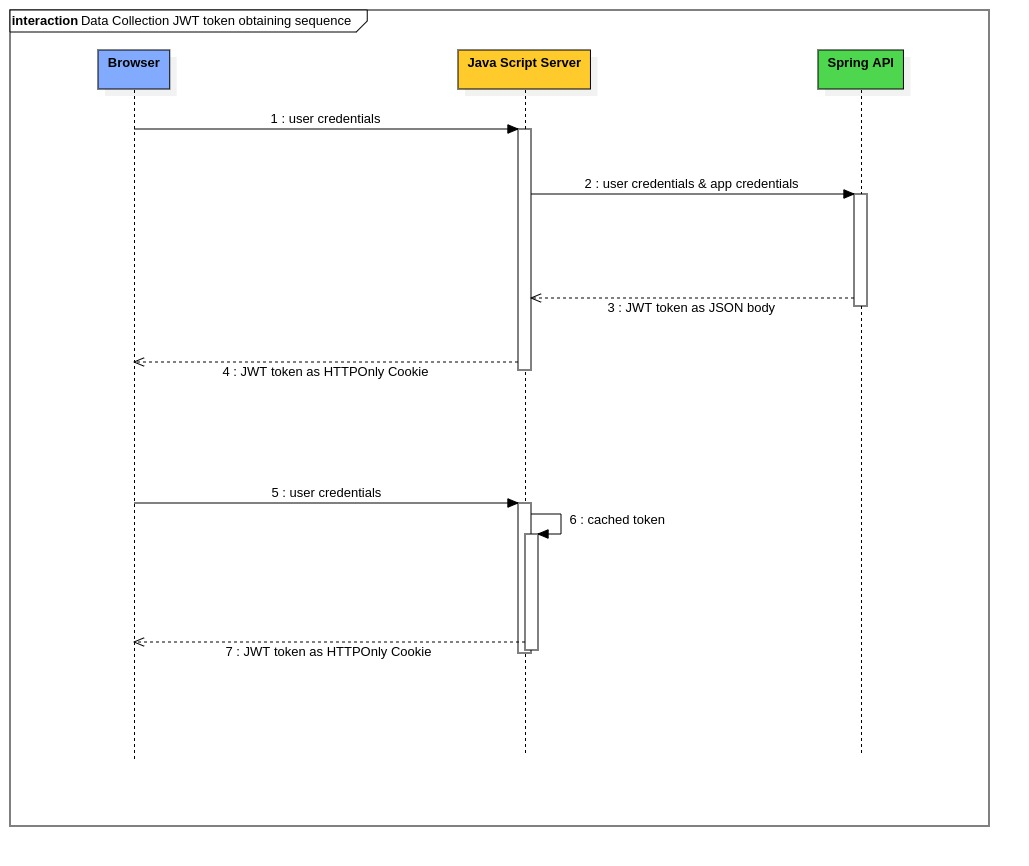
\includegraphics[width=\linewidth]{resources/JWT token obtaining sequence.jpg}
    \captionsetup{width=\linewidth}
    \captionof{figure}{JWT token obtaining sequence}
    \label{fig:jwt-sequence}
\end{figure}

\subsection{Server side module}\label{subsec:server-side-module}
The server side module is build with Node.js\footnote{\url{https://nodejs.org/}} runtime with the Express\footnote{\url{https://expressjs.com/}} framework on the top of it.
Node.js is an asynchronous JavaScript runtime, which is widely used to build high-end, scalable commercial applications.
Express is light-weight, simple to use web framework for Node.js, which allows for conviniently set up a http server for serving the static web documents over the internet.
This module is serving the purpose of reverse proxy between clients and the backend API.

Main responsibilities of this module are:
\begin{enumerate}
    \item User verification --- Tekst tutajTekst tutajTekst tutajTekst tutajTekst tutajTekst tutajTekst tutajTekst tutajTekst tutajTekst tutajTekst tutajTekst tutajTekst tutajTekst tutajTekst tutajTekst tutajTekst tutajTekst tutajTekst tutajTekst tutaj 
    \\ \vspace{-7mm}
    \item Token obtaining --- 
    \\ \vspace{-7mm}
    \item Token validation --- 
    \\ \vspace{-7mm}
    \item Token caching --- 
    \\ \vspace{-7mm}
    \item Serving static web documents --- 
    \\ \vspace{-7mm}
    \item Storing and passing the data for persistence --- \\
\end{enumerate}


